%!TEX root = ../../thesis.tex

The Higgs boson is predicted to have zero spin and positive parity, whilst being 
electrically neutral and colourless. It couples directly to massive particles. Other 
properties, such as production cross sections and \acp{BR} of decay, must be calculated 
as a function of its mass, which is not predicted by the \ac{SM}.

% Experimental signatures for the Higgs boson are categorised according to production 
% mode and decay channel.

At a hadron collider such as the \acs{LHC}, the important production modes are \ac{ggF},
\ac{VBF}, Higgs-strahlung (\WH and \ZH) and top fusion (\ttH). Example Feynman diagrams 
are shown in \Figure~\ref{fig:feyn}. We note that the Higgs boson does not couple to 
massless gluons, therefore \ac{ggF} proceeds via loops of massive coloured particles 
(predominantly the top quark due to its large mass). 

\begin{figure}[b]
	\null\hfill
	\begin{subfigure}[b]{0.4\textwidth}
		\centering
		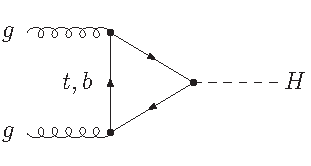
\includegraphics[width=\textwidth]{axodraw/ggF.pdf}
		\caption{Gluon-gluon fusion (ggF)}
		\label{fig:feyn:ggF}
	\end{subfigure}
	\hfill
	\begin{subfigure}[b]{0.4\textwidth}
		\centering
		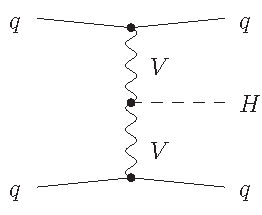
\includegraphics[width=0.75\textwidth]{axodraw/VBF.pdf}
		\caption{Vector boson fusion (VBF)}
		\label{fig:feyn:VBF}
	\end{subfigure}
	\hfill\null
	\\\bigskip
	\null\hfill
	\begin{subfigure}[b]{0.4\textwidth}
		\centering
		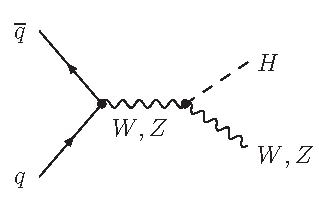
\includegraphics[width=0.8\textwidth]{axodraw/VH.pdf}
		\caption{Higgs-strahlung (\WH and \ZH)}
		\label{fig:feyn:VH}
	\end{subfigure}
	\hfill
	\begin{subfigure}[b]{0.4\textwidth}
		\centering
		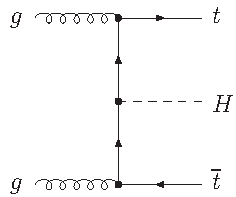
\includegraphics[width=0.625\textwidth]{axodraw/ttH.pdf}
		\caption{Top fusion (\ttH)}
		\label{fig:feyn:ttH}
	\end{subfigure}
	\hfill\null
	\caption{Examples of tree-level Feynman diagrams for the Higgs production processes relevant at the \ac{LHC}.}
	\label{fig:feyn}
\end{figure}

The production cross sections at the \acs{LHC} are shown in \Figure~\ref{fig:higgs_xs}. 
Whilst \ac{ggF} clearly dominates these rare processes, it suffers from large 
experimental backgrounds. The four other modes feature additional final state particles 
which can aid identification. For example, \ac{VBF} has two well-separated quarks with no 
colour exchange between them.

\begin{figure}
	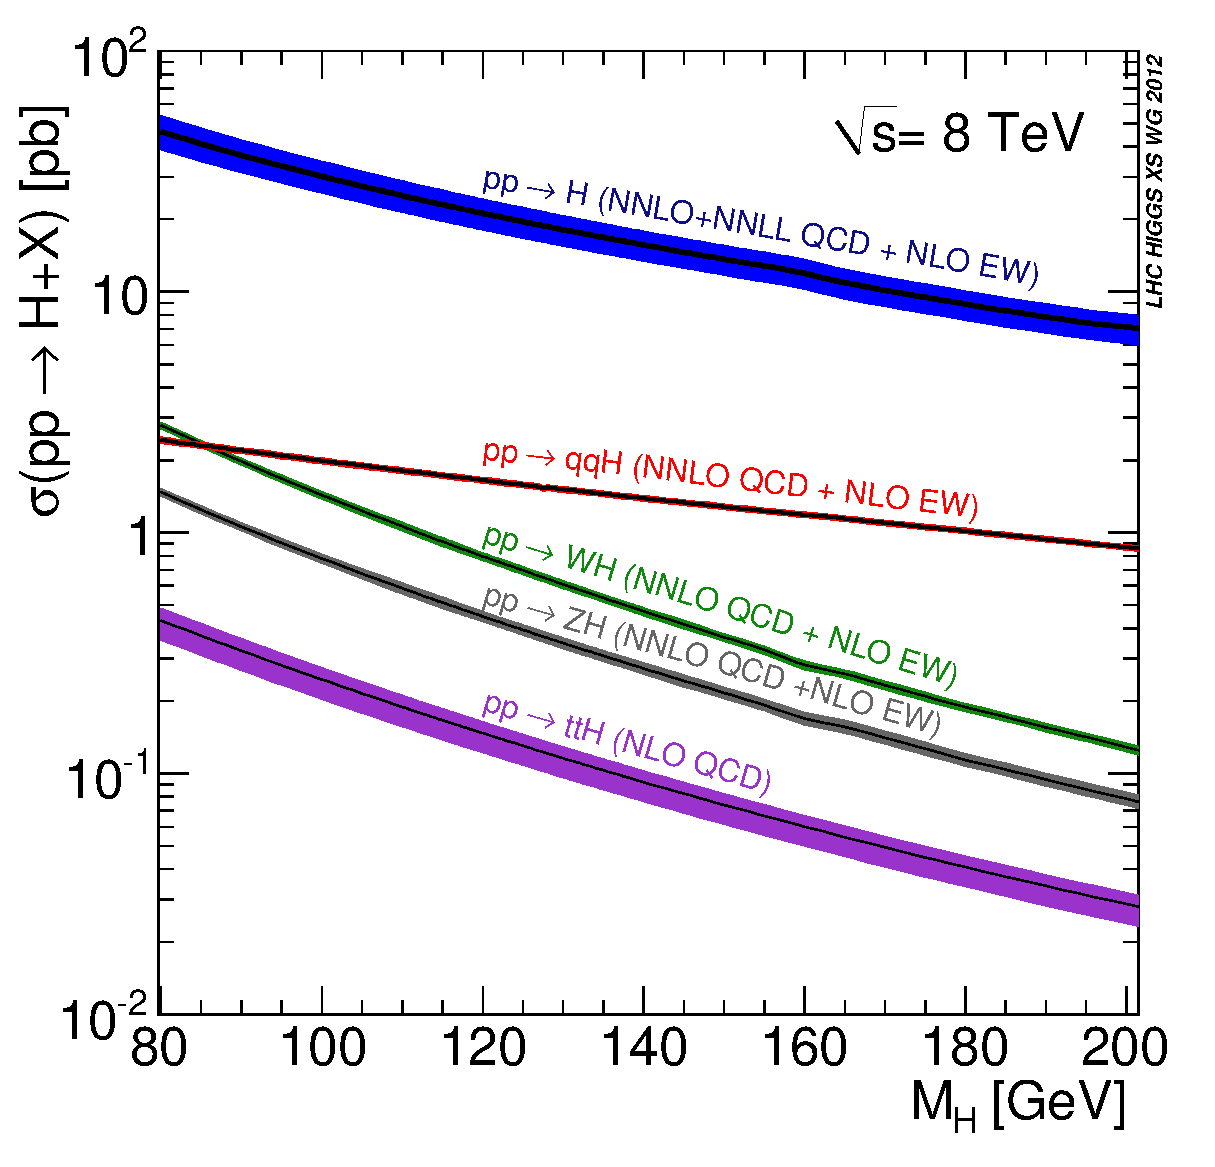
\includegraphics[width=0.48\textwidth]{tex/motivation/xs_lowrange}
	\hfill
	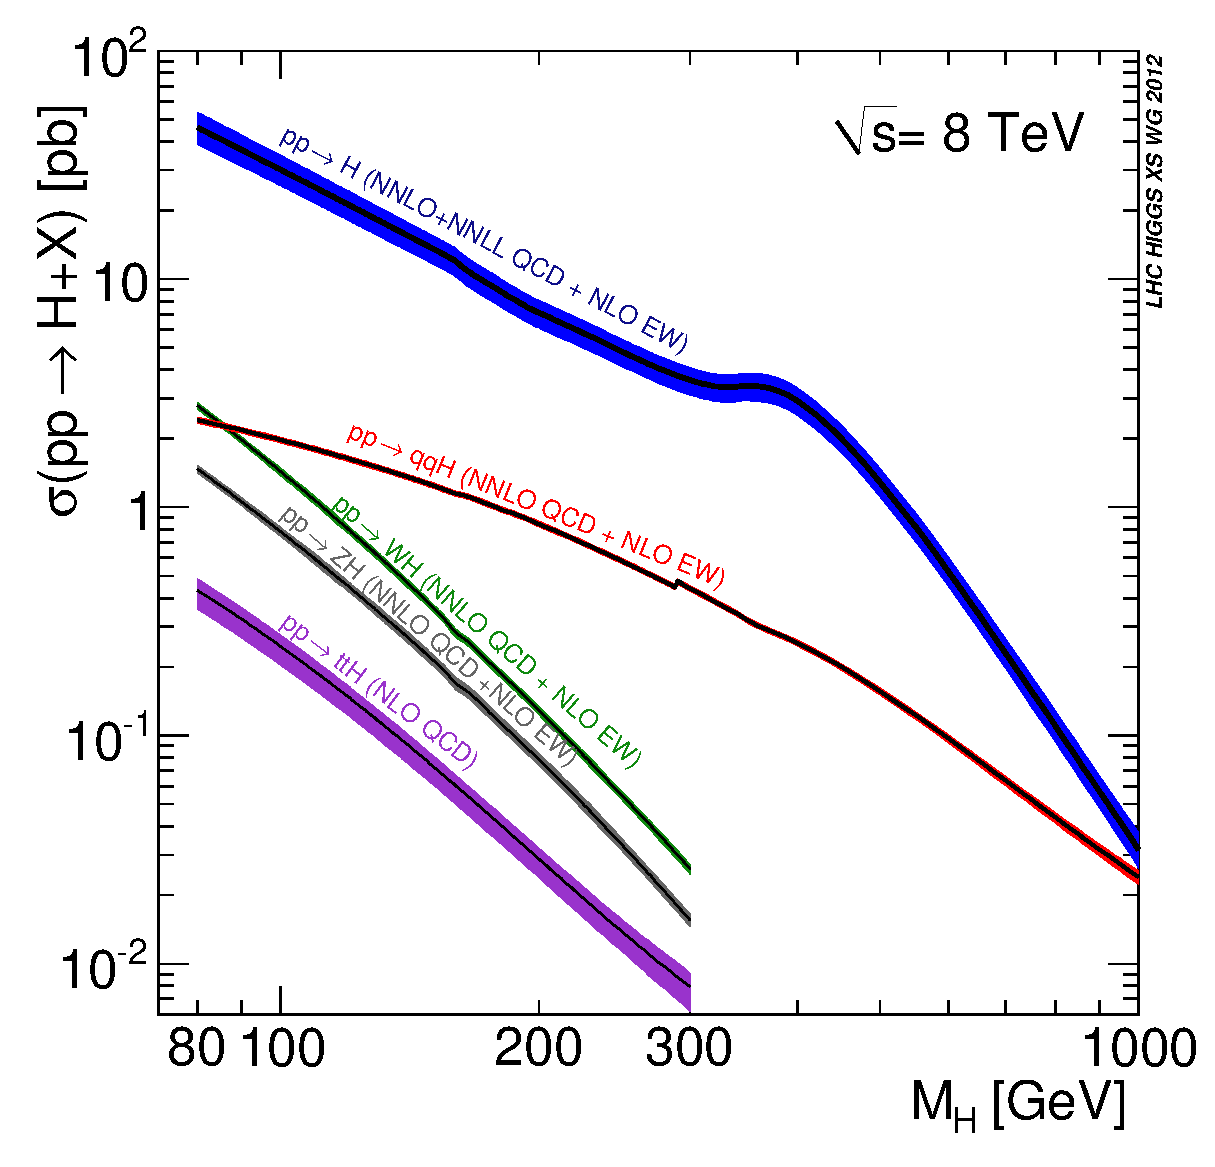
\includegraphics[width=0.48\textwidth]{tex/motivation/xs_fullrange}
	\caption{Higgs boson production cross sections versus mass at 
	\unit{$\sqrt{s} = 8$}{\TeV} for a low mass range (left) and an expanded mass range 
	(right) \cite{YR2}. Theoretical uncertainties are shown as bands. The production modes
	are \ac{ggF} (blue), \ac{VBF} (red), \WH (green), \ZH (grey) and \ttH (purple).}
	\label{fig:higgs_xs}
\end{figure}

Since the lifetime of the Higgs boson is very short, it is never directly observed in a 
detector. Therefore it is important to understand the \acp{BR} of its decays 
(\Figure~\ref{fig:higgs_br}). Na\"{i}vely, these are understood from the Higgs boson coupling to mass and the kinematic requirement $m_{\PHiggs} > m_X + m_Y$ for a decay
\HepProcess{\PHiggs \HepTo XY}. This is complicated by off-shell particles (\eg a low mass
Higgs boson may decay to \HepProcess{\PW \PW^{*}}). 
Also, the \HepProcess{\Pphoton \Pphoton}, \HepProcess{\PZ \Pphoton} and 
\HepProcess{\Pgluon \Pgluon} decay modes are different since they feature massless 
particles, and therefore proceed via loops of massive charged particles (electric charge 
for \HepProcess{\Pphoton \Pphoton} and \HepProcess{\PZ \Pphoton}, colour charge for 
\HepProcess{\Pgluon \Pgluon}).

Designing a sensitive experimental search strategy for the Higgs boson can be difficult. 
In decay channels featuring weak bosons, the subsequent decay of the \PW or \PZ boson must 
also be considered. These are more likely to decay to quarks than to leptons, but the 
former suffers from large backgrounds at hadron colliders. Similarly, the 
\HepProcess{\Pbottom \APbottom} decay has the largest \ac{BR} for low \mH but suffers from 
huge backgrounds. The sensitivity can be improved by combining with a more distinguished 
production mode, such as \WH or \ZH, but this reduces the production cross section.

\begin{figure}
	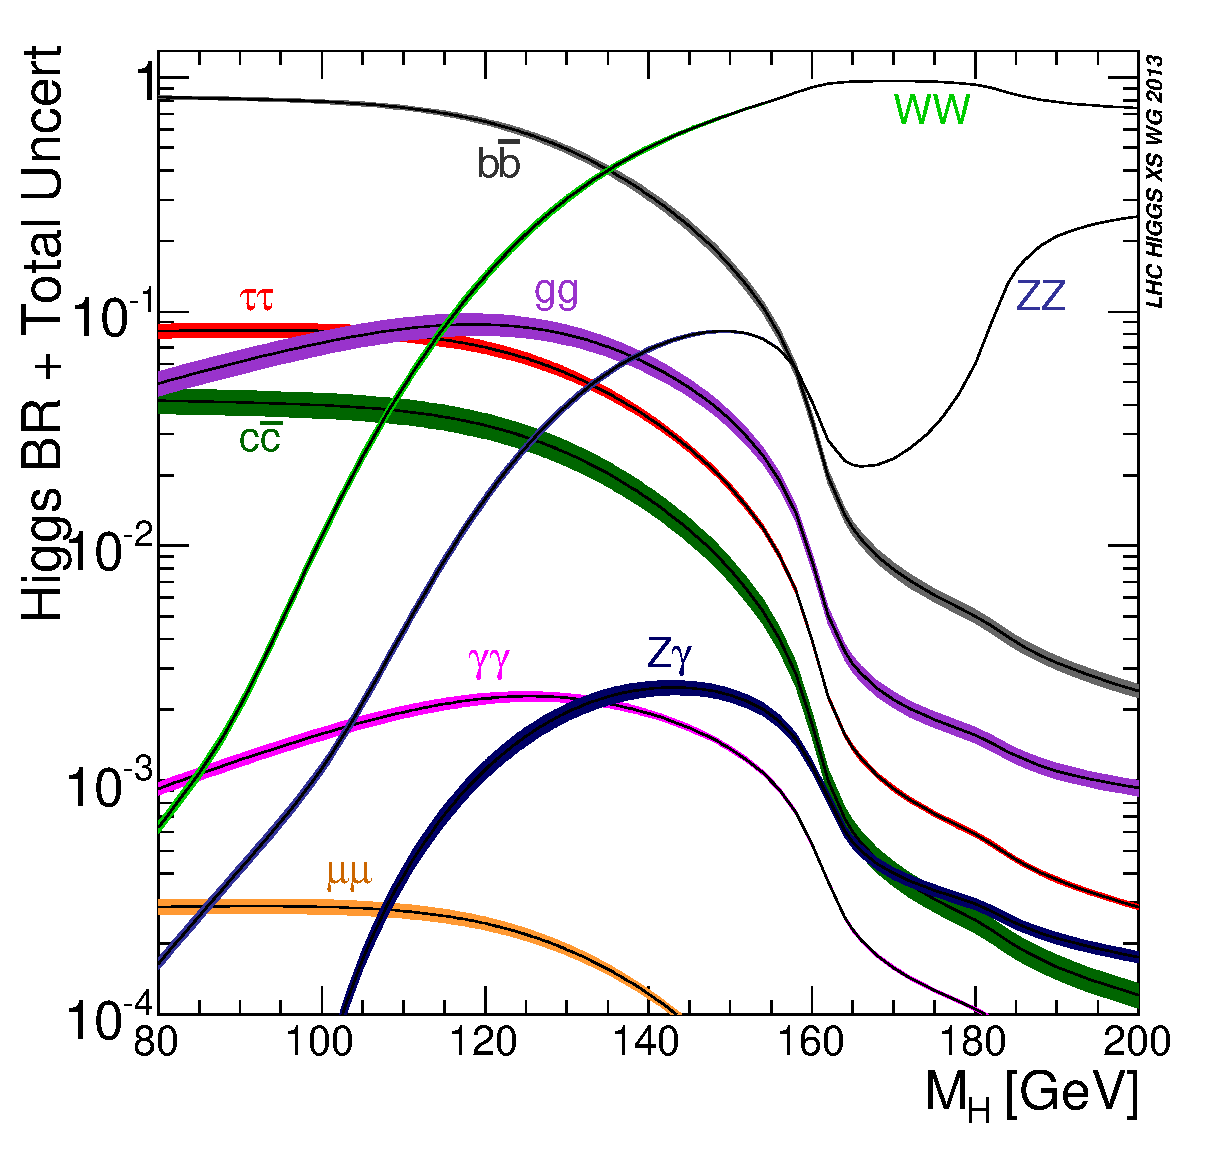
\includegraphics[width=0.48\textwidth]{tex/motivation/BR_lowrange}
	\hfill
	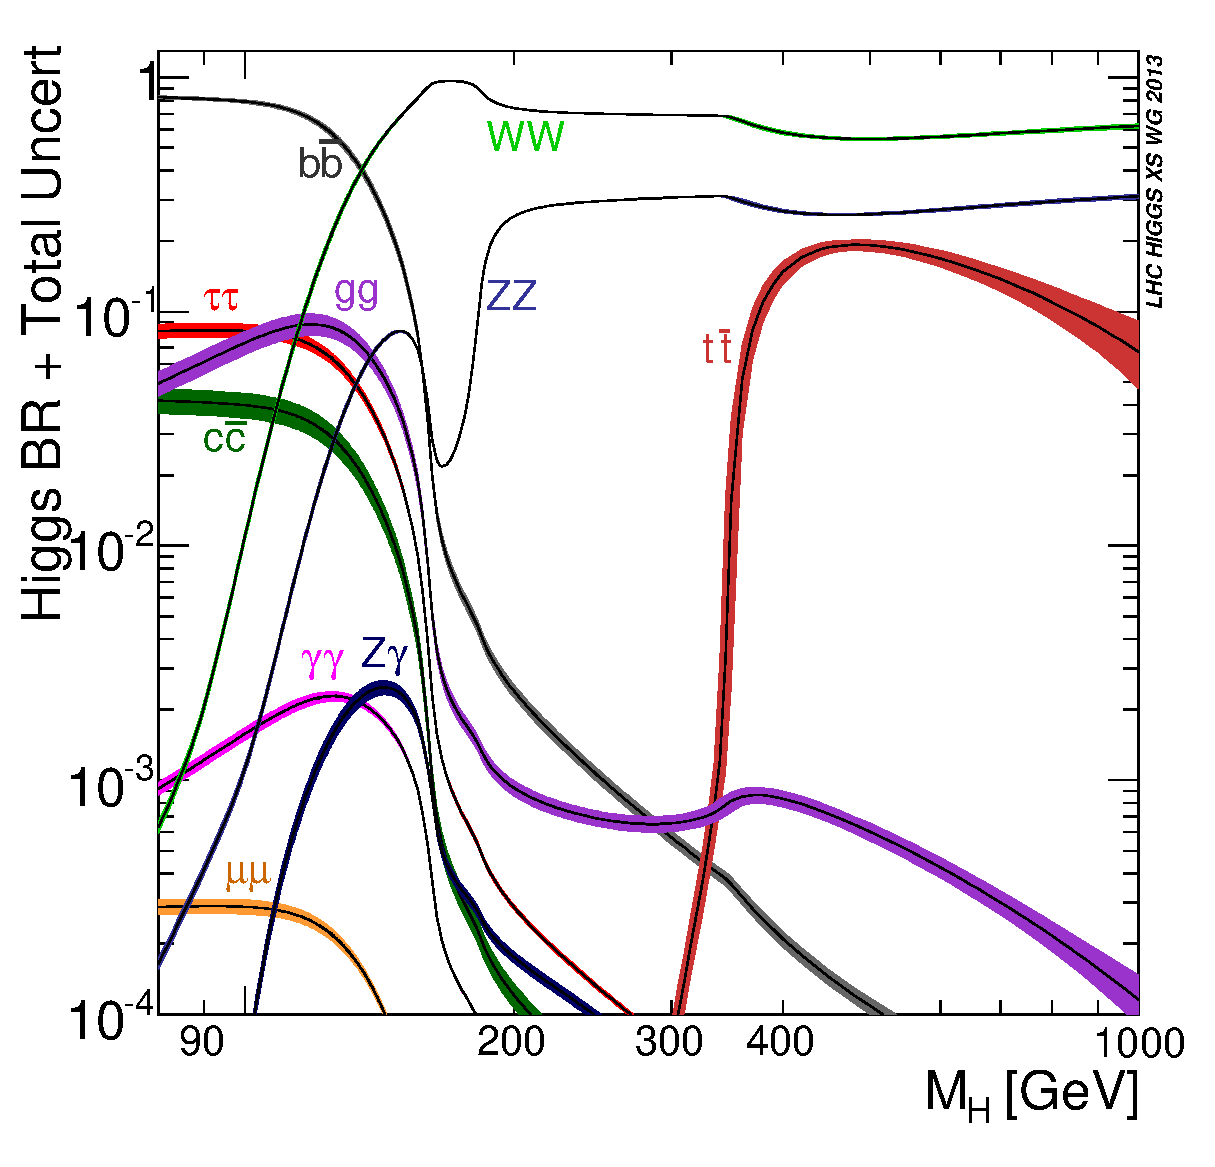
\includegraphics[width=0.48\textwidth]{tex/motivation/BR_fullrange}
	\caption{Branching ratios of Higgs boson decay versus mass for a low mass range (left) 
	and an expanded mass range (right) \cite{YR3}. Theoretical uncertainties are shown as 
	bands.}
	\label{fig:higgs_br}
\end{figure}
